% Options for packages loaded elsewhere
\PassOptionsToPackage{unicode}{hyperref}
\PassOptionsToPackage{hyphens}{url}
%
\documentclass[
]{article}
\usepackage{lmodern}
\usepackage{amssymb,amsmath}
\usepackage{ifxetex,ifluatex}
\ifnum 0\ifxetex 1\fi\ifluatex 1\fi=0 % if pdftex
  \usepackage[T1]{fontenc}
  \usepackage[utf8]{inputenc}
  \usepackage{textcomp} % provide euro and other symbols
\else % if luatex or xetex
  \usepackage{unicode-math}
  \defaultfontfeatures{Scale=MatchLowercase}
  \defaultfontfeatures[\rmfamily]{Ligatures=TeX,Scale=1}
\fi
% Use upquote if available, for straight quotes in verbatim environments
\IfFileExists{upquote.sty}{\usepackage{upquote}}{}
\IfFileExists{microtype.sty}{% use microtype if available
  \usepackage[]{microtype}
  \UseMicrotypeSet[protrusion]{basicmath} % disable protrusion for tt fonts
}{}
\makeatletter
\@ifundefined{KOMAClassName}{% if non-KOMA class
  \IfFileExists{parskip.sty}{%
    \usepackage{parskip}
  }{% else
    \setlength{\parindent}{0pt}
    \setlength{\parskip}{6pt plus 2pt minus 1pt}}
}{% if KOMA class
  \KOMAoptions{parskip=half}}
\makeatother
\usepackage{xcolor}
\IfFileExists{xurl.sty}{\usepackage{xurl}}{} % add URL line breaks if available
\IfFileExists{bookmark.sty}{\usepackage{bookmark}}{\usepackage{hyperref}}
\hypersetup{
  pdftitle={Nightingale\_Coxcomb},
  pdfauthor={coop711},
  hidelinks,
  pdfcreator={LaTeX via pandoc}}
\urlstyle{same} % disable monospaced font for URLs
\usepackage[margin=1in]{geometry}
\usepackage{color}
\usepackage{fancyvrb}
\newcommand{\VerbBar}{|}
\newcommand{\VERB}{\Verb[commandchars=\\\{\}]}
\DefineVerbatimEnvironment{Highlighting}{Verbatim}{commandchars=\\\{\}}
% Add ',fontsize=\small' for more characters per line
\usepackage{framed}
\definecolor{shadecolor}{RGB}{248,248,248}
\newenvironment{Shaded}{\begin{snugshade}}{\end{snugshade}}
\newcommand{\AlertTok}[1]{\textcolor[rgb]{0.94,0.16,0.16}{#1}}
\newcommand{\AnnotationTok}[1]{\textcolor[rgb]{0.56,0.35,0.01}{\textbf{\textit{#1}}}}
\newcommand{\AttributeTok}[1]{\textcolor[rgb]{0.77,0.63,0.00}{#1}}
\newcommand{\BaseNTok}[1]{\textcolor[rgb]{0.00,0.00,0.81}{#1}}
\newcommand{\BuiltInTok}[1]{#1}
\newcommand{\CharTok}[1]{\textcolor[rgb]{0.31,0.60,0.02}{#1}}
\newcommand{\CommentTok}[1]{\textcolor[rgb]{0.56,0.35,0.01}{\textit{#1}}}
\newcommand{\CommentVarTok}[1]{\textcolor[rgb]{0.56,0.35,0.01}{\textbf{\textit{#1}}}}
\newcommand{\ConstantTok}[1]{\textcolor[rgb]{0.00,0.00,0.00}{#1}}
\newcommand{\ControlFlowTok}[1]{\textcolor[rgb]{0.13,0.29,0.53}{\textbf{#1}}}
\newcommand{\DataTypeTok}[1]{\textcolor[rgb]{0.13,0.29,0.53}{#1}}
\newcommand{\DecValTok}[1]{\textcolor[rgb]{0.00,0.00,0.81}{#1}}
\newcommand{\DocumentationTok}[1]{\textcolor[rgb]{0.56,0.35,0.01}{\textbf{\textit{#1}}}}
\newcommand{\ErrorTok}[1]{\textcolor[rgb]{0.64,0.00,0.00}{\textbf{#1}}}
\newcommand{\ExtensionTok}[1]{#1}
\newcommand{\FloatTok}[1]{\textcolor[rgb]{0.00,0.00,0.81}{#1}}
\newcommand{\FunctionTok}[1]{\textcolor[rgb]{0.00,0.00,0.00}{#1}}
\newcommand{\ImportTok}[1]{#1}
\newcommand{\InformationTok}[1]{\textcolor[rgb]{0.56,0.35,0.01}{\textbf{\textit{#1}}}}
\newcommand{\KeywordTok}[1]{\textcolor[rgb]{0.13,0.29,0.53}{\textbf{#1}}}
\newcommand{\NormalTok}[1]{#1}
\newcommand{\OperatorTok}[1]{\textcolor[rgb]{0.81,0.36,0.00}{\textbf{#1}}}
\newcommand{\OtherTok}[1]{\textcolor[rgb]{0.56,0.35,0.01}{#1}}
\newcommand{\PreprocessorTok}[1]{\textcolor[rgb]{0.56,0.35,0.01}{\textit{#1}}}
\newcommand{\RegionMarkerTok}[1]{#1}
\newcommand{\SpecialCharTok}[1]{\textcolor[rgb]{0.00,0.00,0.00}{#1}}
\newcommand{\SpecialStringTok}[1]{\textcolor[rgb]{0.31,0.60,0.02}{#1}}
\newcommand{\StringTok}[1]{\textcolor[rgb]{0.31,0.60,0.02}{#1}}
\newcommand{\VariableTok}[1]{\textcolor[rgb]{0.00,0.00,0.00}{#1}}
\newcommand{\VerbatimStringTok}[1]{\textcolor[rgb]{0.31,0.60,0.02}{#1}}
\newcommand{\WarningTok}[1]{\textcolor[rgb]{0.56,0.35,0.01}{\textbf{\textit{#1}}}}
\usepackage{longtable,booktabs}
% Correct order of tables after \paragraph or \subparagraph
\usepackage{etoolbox}
\makeatletter
\patchcmd\longtable{\par}{\if@noskipsec\mbox{}\fi\par}{}{}
\makeatother
% Allow footnotes in longtable head/foot
\IfFileExists{footnotehyper.sty}{\usepackage{footnotehyper}}{\usepackage{footnote}}
\makesavenoteenv{longtable}
\usepackage{graphicx,grffile}
\makeatletter
\def\maxwidth{\ifdim\Gin@nat@width>\linewidth\linewidth\else\Gin@nat@width\fi}
\def\maxheight{\ifdim\Gin@nat@height>\textheight\textheight\else\Gin@nat@height\fi}
\makeatother
% Scale images if necessary, so that they will not overflow the page
% margins by default, and it is still possible to overwrite the defaults
% using explicit options in \includegraphics[width, height, ...]{}
\setkeys{Gin}{width=\maxwidth,height=\maxheight,keepaspectratio}
% Set default figure placement to htbp
\makeatletter
\def\fps@figure{htbp}
\makeatother
\setlength{\emergencystretch}{3em} % prevent overfull lines
\providecommand{\tightlist}{%
  \setlength{\itemsep}{0pt}\setlength{\parskip}{0pt}}
\setcounter{secnumdepth}{-\maxdimen} % remove section numbering

\title{Nightingale\_Coxcomb}
\author{coop711}
\date{2021-02-10}

\begin{document}
\maketitle

\hypertarget{uxc790uxb8ccuxc640-uxbc30uxacbd}{%
\section{자료와 배경}\label{uxc790uxb8ccuxc640-uxbc30uxacbd}}

나이팅게일(Florence Nightingale, 1820-1910)은 크림전쟁(1854-1856) 당시
38명의 잉글랜드 성공회 수녀들의 도움을 받으며 슈코더르(Scutari)의 야전
병원에서 유능한 보건행정가로서의 역량을 발휘하여 병원에서 쓰는 물건을
세심하게 관리하고 무질서한 병원에 규율을 세웠다. 환자의 사망율을
42\%에서 2\%로 낮추고 집중치료실(ICU)을 설치하여 상태가 중한 환자를
격리하여 집중관리하는 등 근대적인 간호체계를 수립하는 데 기여하였다.
관료주의에 물든 군의 관리들을 설득하기 위하여 사용한 다음 도표는 Rose
Diagram, 혹은 Coxcomb plot 등으로 불린다.

\begin{Shaded}
\begin{Highlighting}[]
\NormalTok{knitr}\OperatorTok{::}\KeywordTok{include_graphics}\NormalTok{(}\StringTok{"../pics/Nightingale_Coxcomb.jpg"}\NormalTok{)}
\end{Highlighting}
\end{Shaded}

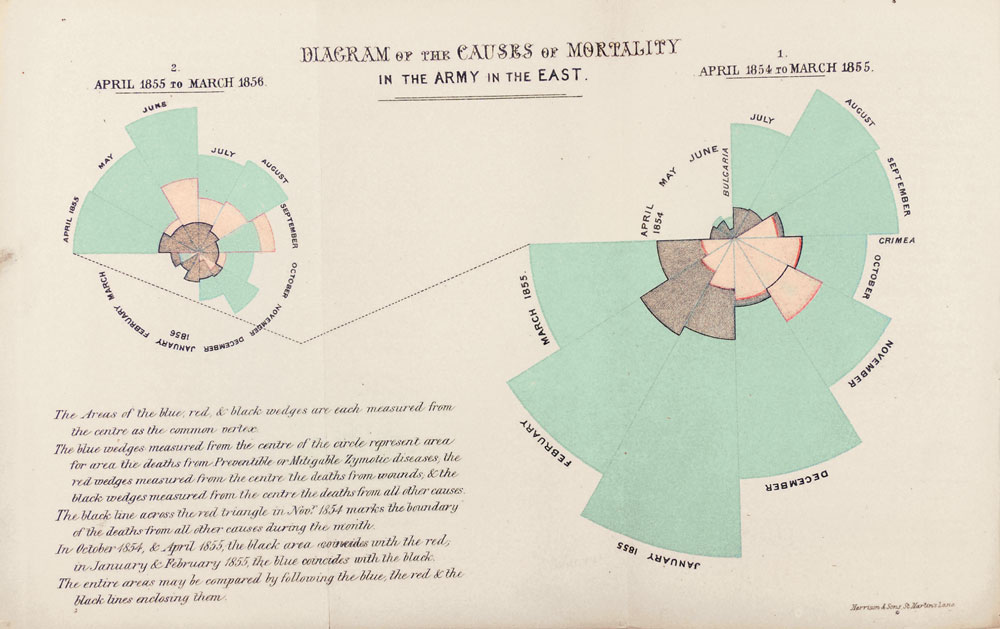
\includegraphics[width=1\linewidth]{../pics/Nightingale_Coxcomb}

\hypertarget{uxb370uxc774uxd130}{%
\section{데이터}\label{uxb370uxc774uxd130}}

\begin{Shaded}
\begin{Highlighting}[]
\KeywordTok{library}\NormalTok{(knitr)}
\KeywordTok{library}\NormalTok{(HistData)}
\KeywordTok{library}\NormalTok{(tidyverse)}
\KeywordTok{library}\NormalTok{(magrittr)}
\KeywordTok{library}\NormalTok{(grid)}
\KeywordTok{library}\NormalTok{(gridExtra)}
\KeywordTok{kable}\NormalTok{(Nightingale)}
\end{Highlighting}
\end{Shaded}

\begin{longtable}[]{@{}llrrrrrrrr@{}}
\toprule
Date & Month & Year & Army & Disease & Wounds & Other & Disease.rate &
Wounds.rate & Other.rate\tabularnewline
\midrule
\endhead
1854-04-01 & Apr & 1854 & 8571 & 1 & 0 & 5 & 1.4 & 0.0 &
7.0\tabularnewline
1854-05-01 & May & 1854 & 23333 & 12 & 0 & 9 & 6.2 & 0.0 &
4.6\tabularnewline
1854-06-01 & Jun & 1854 & 28333 & 11 & 0 & 6 & 4.7 & 0.0 &
2.5\tabularnewline
1854-07-01 & Jul & 1854 & 28722 & 359 & 0 & 23 & 150.0 & 0.0 &
9.6\tabularnewline
1854-08-01 & Aug & 1854 & 30246 & 828 & 1 & 30 & 328.5 & 0.4 &
11.9\tabularnewline
1854-09-01 & Sep & 1854 & 30290 & 788 & 81 & 70 & 312.2 & 32.1 &
27.7\tabularnewline
1854-10-01 & Oct & 1854 & 30643 & 503 & 132 & 128 & 197.0 & 51.7 &
50.1\tabularnewline
1854-11-01 & Nov & 1854 & 29736 & 844 & 287 & 106 & 340.6 & 115.8 &
42.8\tabularnewline
1854-12-01 & Dec & 1854 & 32779 & 1725 & 114 & 131 & 631.5 & 41.7 &
48.0\tabularnewline
1855-01-01 & Jan & 1855 & 32393 & 2761 & 83 & 324 & 1022.8 & 30.7 &
120.0\tabularnewline
1855-02-01 & Feb & 1855 & 30919 & 2120 & 42 & 361 & 822.8 & 16.3 &
140.1\tabularnewline
1855-03-01 & Mar & 1855 & 30107 & 1205 & 32 & 172 & 480.3 & 12.8 &
68.6\tabularnewline
1855-04-01 & Apr & 1855 & 32252 & 477 & 48 & 57 & 177.5 & 17.9 &
21.2\tabularnewline
1855-05-01 & May & 1855 & 35473 & 508 & 49 & 37 & 171.8 & 16.6 &
12.5\tabularnewline
1855-06-01 & Jun & 1855 & 38863 & 802 & 209 & 31 & 247.6 & 64.5 &
9.6\tabularnewline
1855-07-01 & Jul & 1855 & 42647 & 382 & 134 & 33 & 107.5 & 37.7 &
9.3\tabularnewline
1855-08-01 & Aug & 1855 & 44614 & 483 & 164 & 25 & 129.9 & 44.1 &
6.7\tabularnewline
1855-09-01 & Sep & 1855 & 47751 & 189 & 276 & 20 & 47.5 & 69.4 &
5.0\tabularnewline
1855-10-01 & Oct & 1855 & 46852 & 128 & 53 & 18 & 32.8 & 13.6 &
4.6\tabularnewline
1855-11-01 & Nov & 1855 & 37853 & 178 & 33 & 32 & 56.4 & 10.5 &
10.1\tabularnewline
1855-12-01 & Dec & 1855 & 43217 & 91 & 18 & 28 & 25.3 & 5.0 &
7.8\tabularnewline
1856-01-01 & Jan & 1856 & 44212 & 42 & 2 & 48 & 11.4 & 0.5 &
13.0\tabularnewline
1856-02-01 & Feb & 1856 & 43485 & 24 & 0 & 19 & 6.6 & 0.0 &
5.2\tabularnewline
1856-03-01 & Mar & 1856 & 46140 & 15 & 0 & 35 & 3.9 & 0.0 &
9.1\tabularnewline
\bottomrule
\end{longtable}

\begin{Shaded}
\begin{Highlighting}[]
\NormalTok{Night <-}\StringTok{ }\NormalTok{Nightingale }\OperatorTok
\StringTok{  }\NormalTok{as_tibble }\OperatorTok
\StringTok{  }\KeywordTok{subset}\NormalTok{(}\DataTypeTok{select =} \KeywordTok{c}\NormalTok{(}\DecValTok{1}\NormalTok{, }\DecValTok{8}\OperatorTok{:}\DecValTok{10}\NormalTok{))}
\KeywordTok{kable}\NormalTok{(Night)}
\end{Highlighting}
\end{Shaded}

\begin{longtable}[]{@{}lrrr@{}}
\toprule
Date & Disease.rate & Wounds.rate & Other.rate\tabularnewline
\midrule
\endhead
1854-04-01 & 1.4 & 0.0 & 7.0\tabularnewline
1854-05-01 & 6.2 & 0.0 & 4.6\tabularnewline
1854-06-01 & 4.7 & 0.0 & 2.5\tabularnewline
1854-07-01 & 150.0 & 0.0 & 9.6\tabularnewline
1854-08-01 & 328.5 & 0.4 & 11.9\tabularnewline
1854-09-01 & 312.2 & 32.1 & 27.7\tabularnewline
1854-10-01 & 197.0 & 51.7 & 50.1\tabularnewline
1854-11-01 & 340.6 & 115.8 & 42.8\tabularnewline
1854-12-01 & 631.5 & 41.7 & 48.0\tabularnewline
1855-01-01 & 1022.8 & 30.7 & 120.0\tabularnewline
1855-02-01 & 822.8 & 16.3 & 140.1\tabularnewline
1855-03-01 & 480.3 & 12.8 & 68.6\tabularnewline
1855-04-01 & 177.5 & 17.9 & 21.2\tabularnewline
1855-05-01 & 171.8 & 16.6 & 12.5\tabularnewline
1855-06-01 & 247.6 & 64.5 & 9.6\tabularnewline
1855-07-01 & 107.5 & 37.7 & 9.3\tabularnewline
1855-08-01 & 129.9 & 44.1 & 6.7\tabularnewline
1855-09-01 & 47.5 & 69.4 & 5.0\tabularnewline
1855-10-01 & 32.8 & 13.6 & 4.6\tabularnewline
1855-11-01 & 56.4 & 10.5 & 10.1\tabularnewline
1855-12-01 & 25.3 & 5.0 & 7.8\tabularnewline
1856-01-01 & 11.4 & 0.5 & 13.0\tabularnewline
1856-02-01 & 6.6 & 0.0 & 5.2\tabularnewline
1856-03-01 & 3.9 & 0.0 & 9.1\tabularnewline
\bottomrule
\end{longtable}

\begin{Shaded}
\begin{Highlighting}[]
\NormalTok{Night }\OperatorTok
\StringTok{  }\KeywordTok{gather}\NormalTok{(}\DataTypeTok{key =} \StringTok{"Cause"}\NormalTok{, }\DataTypeTok{value =} \StringTok{"Deaths"}\NormalTok{, }\OperatorTok{-}\NormalTok{Date) }\OperatorTok
\StringTok{  }\KeywordTok{mutate}\NormalTok{(}\DataTypeTok{Month =} \KeywordTok{gl}\NormalTok{(}\DecValTok{12}\NormalTok{, }\DecValTok{1}\NormalTok{, }\DecValTok{72}\NormalTok{, }\DataTypeTok{labels =}\NormalTok{ month.name[}\KeywordTok{c}\NormalTok{(}\DecValTok{4}\OperatorTok{:}\DecValTok{12}\NormalTok{, }\DecValTok{1}\OperatorTok{:}\DecValTok{3}\NormalTok{)])) }\OperatorTok
\StringTok{  }\KeywordTok{mutate}\NormalTok{(}\DataTypeTok{Regime =} \KeywordTok{gl}\NormalTok{(}\DecValTok{2}\NormalTok{, }\DecValTok{12}\NormalTok{, }\DecValTok{72}\NormalTok{, }\DataTypeTok{labels =} \KeywordTok{c}\NormalTok{(}\StringTok{"Before"}\NormalTok{, }\StringTok{"After"}\NormalTok{), }\DataTypeTok{ordered =} \OtherTok{TRUE}\NormalTok{)) }
\KeywordTok{kable}\NormalTok{(Night)}
\end{Highlighting}
\end{Shaded}

\begin{longtable}[]{@{}llrll@{}}
\toprule
Date & Cause & Deaths & Month & Regime\tabularnewline
\midrule
\endhead
1854-04-01 & Disease.rate & 1.4 & April & Before\tabularnewline
1854-05-01 & Disease.rate & 6.2 & May & Before\tabularnewline
1854-06-01 & Disease.rate & 4.7 & June & Before\tabularnewline
1854-07-01 & Disease.rate & 150.0 & July & Before\tabularnewline
1854-08-01 & Disease.rate & 328.5 & August & Before\tabularnewline
1854-09-01 & Disease.rate & 312.2 & September & Before\tabularnewline
1854-10-01 & Disease.rate & 197.0 & October & Before\tabularnewline
1854-11-01 & Disease.rate & 340.6 & November & Before\tabularnewline
1854-12-01 & Disease.rate & 631.5 & December & Before\tabularnewline
1855-01-01 & Disease.rate & 1022.8 & January & Before\tabularnewline
1855-02-01 & Disease.rate & 822.8 & February & Before\tabularnewline
1855-03-01 & Disease.rate & 480.3 & March & Before\tabularnewline
1855-04-01 & Disease.rate & 177.5 & April & After\tabularnewline
1855-05-01 & Disease.rate & 171.8 & May & After\tabularnewline
1855-06-01 & Disease.rate & 247.6 & June & After\tabularnewline
1855-07-01 & Disease.rate & 107.5 & July & After\tabularnewline
1855-08-01 & Disease.rate & 129.9 & August & After\tabularnewline
1855-09-01 & Disease.rate & 47.5 & September & After\tabularnewline
1855-10-01 & Disease.rate & 32.8 & October & After\tabularnewline
1855-11-01 & Disease.rate & 56.4 & November & After\tabularnewline
1855-12-01 & Disease.rate & 25.3 & December & After\tabularnewline
1856-01-01 & Disease.rate & 11.4 & January & After\tabularnewline
1856-02-01 & Disease.rate & 6.6 & February & After\tabularnewline
1856-03-01 & Disease.rate & 3.9 & March & After\tabularnewline
1854-04-01 & Wounds.rate & 0.0 & April & Before\tabularnewline
1854-05-01 & Wounds.rate & 0.0 & May & Before\tabularnewline
1854-06-01 & Wounds.rate & 0.0 & June & Before\tabularnewline
1854-07-01 & Wounds.rate & 0.0 & July & Before\tabularnewline
1854-08-01 & Wounds.rate & 0.4 & August & Before\tabularnewline
1854-09-01 & Wounds.rate & 32.1 & September & Before\tabularnewline
1854-10-01 & Wounds.rate & 51.7 & October & Before\tabularnewline
1854-11-01 & Wounds.rate & 115.8 & November & Before\tabularnewline
1854-12-01 & Wounds.rate & 41.7 & December & Before\tabularnewline
1855-01-01 & Wounds.rate & 30.7 & January & Before\tabularnewline
1855-02-01 & Wounds.rate & 16.3 & February & Before\tabularnewline
1855-03-01 & Wounds.rate & 12.8 & March & Before\tabularnewline
1855-04-01 & Wounds.rate & 17.9 & April & After\tabularnewline
1855-05-01 & Wounds.rate & 16.6 & May & After\tabularnewline
1855-06-01 & Wounds.rate & 64.5 & June & After\tabularnewline
1855-07-01 & Wounds.rate & 37.7 & July & After\tabularnewline
1855-08-01 & Wounds.rate & 44.1 & August & After\tabularnewline
1855-09-01 & Wounds.rate & 69.4 & September & After\tabularnewline
1855-10-01 & Wounds.rate & 13.6 & October & After\tabularnewline
1855-11-01 & Wounds.rate & 10.5 & November & After\tabularnewline
1855-12-01 & Wounds.rate & 5.0 & December & After\tabularnewline
1856-01-01 & Wounds.rate & 0.5 & January & After\tabularnewline
1856-02-01 & Wounds.rate & 0.0 & February & After\tabularnewline
1856-03-01 & Wounds.rate & 0.0 & March & After\tabularnewline
1854-04-01 & Other.rate & 7.0 & April & Before\tabularnewline
1854-05-01 & Other.rate & 4.6 & May & Before\tabularnewline
1854-06-01 & Other.rate & 2.5 & June & Before\tabularnewline
1854-07-01 & Other.rate & 9.6 & July & Before\tabularnewline
1854-08-01 & Other.rate & 11.9 & August & Before\tabularnewline
1854-09-01 & Other.rate & 27.7 & September & Before\tabularnewline
1854-10-01 & Other.rate & 50.1 & October & Before\tabularnewline
1854-11-01 & Other.rate & 42.8 & November & Before\tabularnewline
1854-12-01 & Other.rate & 48.0 & December & Before\tabularnewline
1855-01-01 & Other.rate & 120.0 & January & Before\tabularnewline
1855-02-01 & Other.rate & 140.1 & February & Before\tabularnewline
1855-03-01 & Other.rate & 68.6 & March & Before\tabularnewline
1855-04-01 & Other.rate & 21.2 & April & After\tabularnewline
1855-05-01 & Other.rate & 12.5 & May & After\tabularnewline
1855-06-01 & Other.rate & 9.6 & June & After\tabularnewline
1855-07-01 & Other.rate & 9.3 & July & After\tabularnewline
1855-08-01 & Other.rate & 6.7 & August & After\tabularnewline
1855-09-01 & Other.rate & 5.0 & September & After\tabularnewline
1855-10-01 & Other.rate & 4.6 & October & After\tabularnewline
1855-11-01 & Other.rate & 10.1 & November & After\tabularnewline
1855-12-01 & Other.rate & 7.8 & December & After\tabularnewline
1856-01-01 & Other.rate & 13.0 & January & After\tabularnewline
1856-02-01 & Other.rate & 5.2 & February & After\tabularnewline
1856-03-01 & Other.rate & 9.1 & March & After\tabularnewline
\bottomrule
\end{longtable}

\begin{Shaded}
\begin{Highlighting}[]
\KeywordTok{str}\NormalTok{(Night)}
\end{Highlighting}
\end{Shaded}

\begin{verbatim}
## tibble [72 x 5] (S3: tbl_df/tbl/data.frame)
##  $ Date  : Date[1:72], format: "1854-04-01" "1854-05-01" ...
##  $ Cause : chr [1:72] "Disease.rate" "Disease.rate" "Disease.rate" "Disease.rate" ...
##  $ Deaths: num [1:72] 1.4 6.2 4.7 150 328.5 ...
##  $ Month : Factor w/ 12 levels "April","May",..: 1 2 3 4 5 6 7 8 9 10 ...
##  $ Regime: Ord.factor w/ 2 levels "Before"<"After": 1 1 1 1 1 1 1 1 1 1 ...
\end{verbatim}

\begin{Shaded}
\begin{Highlighting}[]
\NormalTok{Night}\OperatorTok{$}\NormalTok{Cause }\OperatorTok\StringTok{ }
\StringTok{  }\KeywordTok{sub}\NormalTok{(}\StringTok{"}\CharTok{\textbackslash{}\textbackslash{}}\StringTok{.rate"}\NormalTok{, }\StringTok{""}\NormalTok{, .)}
\NormalTok{Night}\OperatorTok{$}\NormalTok{Cause }\OperatorTok\StringTok{ }
\StringTok{  }\KeywordTok{factor}\NormalTok{(}\DataTypeTok{levels =} \KeywordTok{c}\NormalTok{(}\StringTok{"Disease"}\NormalTok{, }\StringTok{"Wounds"}\NormalTok{, }\StringTok{"Other"}\NormalTok{))}
\NormalTok{Night }\OperatorTok
\StringTok{  }\KeywordTok{kable}\NormalTok{(}\DataTypeTok{align =} \KeywordTok{c}\NormalTok{(}\StringTok{"c"}\NormalTok{, }\StringTok{"c"}\NormalTok{, }\StringTok{"r"}\NormalTok{, }\StringTok{"c"}\NormalTok{, }\StringTok{"c"}\NormalTok{))}
\end{Highlighting}
\end{Shaded}

\begin{longtable}[]{@{}ccrcc@{}}
\toprule
Date & Cause & Deaths & Month & Regime\tabularnewline
\midrule
\endhead
1854-04-01 & Disease & 1.4 & April & Before\tabularnewline
1854-05-01 & Disease & 6.2 & May & Before\tabularnewline
1854-06-01 & Disease & 4.7 & June & Before\tabularnewline
1854-07-01 & Disease & 150.0 & July & Before\tabularnewline
1854-08-01 & Disease & 328.5 & August & Before\tabularnewline
1854-09-01 & Disease & 312.2 & September & Before\tabularnewline
1854-10-01 & Disease & 197.0 & October & Before\tabularnewline
1854-11-01 & Disease & 340.6 & November & Before\tabularnewline
1854-12-01 & Disease & 631.5 & December & Before\tabularnewline
1855-01-01 & Disease & 1022.8 & January & Before\tabularnewline
1855-02-01 & Disease & 822.8 & February & Before\tabularnewline
1855-03-01 & Disease & 480.3 & March & Before\tabularnewline
1855-04-01 & Disease & 177.5 & April & After\tabularnewline
1855-05-01 & Disease & 171.8 & May & After\tabularnewline
1855-06-01 & Disease & 247.6 & June & After\tabularnewline
1855-07-01 & Disease & 107.5 & July & After\tabularnewline
1855-08-01 & Disease & 129.9 & August & After\tabularnewline
1855-09-01 & Disease & 47.5 & September & After\tabularnewline
1855-10-01 & Disease & 32.8 & October & After\tabularnewline
1855-11-01 & Disease & 56.4 & November & After\tabularnewline
1855-12-01 & Disease & 25.3 & December & After\tabularnewline
1856-01-01 & Disease & 11.4 & January & After\tabularnewline
1856-02-01 & Disease & 6.6 & February & After\tabularnewline
1856-03-01 & Disease & 3.9 & March & After\tabularnewline
1854-04-01 & Wounds & 0.0 & April & Before\tabularnewline
1854-05-01 & Wounds & 0.0 & May & Before\tabularnewline
1854-06-01 & Wounds & 0.0 & June & Before\tabularnewline
1854-07-01 & Wounds & 0.0 & July & Before\tabularnewline
1854-08-01 & Wounds & 0.4 & August & Before\tabularnewline
1854-09-01 & Wounds & 32.1 & September & Before\tabularnewline
1854-10-01 & Wounds & 51.7 & October & Before\tabularnewline
1854-11-01 & Wounds & 115.8 & November & Before\tabularnewline
1854-12-01 & Wounds & 41.7 & December & Before\tabularnewline
1855-01-01 & Wounds & 30.7 & January & Before\tabularnewline
1855-02-01 & Wounds & 16.3 & February & Before\tabularnewline
1855-03-01 & Wounds & 12.8 & March & Before\tabularnewline
1855-04-01 & Wounds & 17.9 & April & After\tabularnewline
1855-05-01 & Wounds & 16.6 & May & After\tabularnewline
1855-06-01 & Wounds & 64.5 & June & After\tabularnewline
1855-07-01 & Wounds & 37.7 & July & After\tabularnewline
1855-08-01 & Wounds & 44.1 & August & After\tabularnewline
1855-09-01 & Wounds & 69.4 & September & After\tabularnewline
1855-10-01 & Wounds & 13.6 & October & After\tabularnewline
1855-11-01 & Wounds & 10.5 & November & After\tabularnewline
1855-12-01 & Wounds & 5.0 & December & After\tabularnewline
1856-01-01 & Wounds & 0.5 & January & After\tabularnewline
1856-02-01 & Wounds & 0.0 & February & After\tabularnewline
1856-03-01 & Wounds & 0.0 & March & After\tabularnewline
1854-04-01 & Other & 7.0 & April & Before\tabularnewline
1854-05-01 & Other & 4.6 & May & Before\tabularnewline
1854-06-01 & Other & 2.5 & June & Before\tabularnewline
1854-07-01 & Other & 9.6 & July & Before\tabularnewline
1854-08-01 & Other & 11.9 & August & Before\tabularnewline
1854-09-01 & Other & 27.7 & September & Before\tabularnewline
1854-10-01 & Other & 50.1 & October & Before\tabularnewline
1854-11-01 & Other & 42.8 & November & Before\tabularnewline
1854-12-01 & Other & 48.0 & December & Before\tabularnewline
1855-01-01 & Other & 120.0 & January & Before\tabularnewline
1855-02-01 & Other & 140.1 & February & Before\tabularnewline
1855-03-01 & Other & 68.6 & March & Before\tabularnewline
1855-04-01 & Other & 21.2 & April & After\tabularnewline
1855-05-01 & Other & 12.5 & May & After\tabularnewline
1855-06-01 & Other & 9.6 & June & After\tabularnewline
1855-07-01 & Other & 9.3 & July & After\tabularnewline
1855-08-01 & Other & 6.7 & August & After\tabularnewline
1855-09-01 & Other & 5.0 & September & After\tabularnewline
1855-10-01 & Other & 4.6 & October & After\tabularnewline
1855-11-01 & Other & 10.1 & November & After\tabularnewline
1855-12-01 & Other & 7.8 & December & After\tabularnewline
1856-01-01 & Other & 13.0 & January & After\tabularnewline
1856-02-01 & Other & 5.2 & February & After\tabularnewline
1856-03-01 & Other & 9.1 & March & After\tabularnewline
\bottomrule
\end{longtable}

\hypertarget{plot}{%
\section{Plot}\label{plot}}

\hypertarget{barplot}{%
\subsection{barplot}\label{barplot}}

\begin{Shaded}
\begin{Highlighting}[]
\NormalTok{cxc_b <-}\StringTok{ }
\StringTok{  }\KeywordTok{ggplot}\NormalTok{(}\DataTypeTok{data =}\NormalTok{ Night,}
         \DataTypeTok{mapping =} \KeywordTok{aes}\NormalTok{(}\DataTypeTok{x =} \KeywordTok{factor}\NormalTok{(Date), }
                       \DataTypeTok{y =}\NormalTok{ Deaths, }
                       \DataTypeTok{fill =}\NormalTok{ Cause)) }\OperatorTok{+}
\StringTok{  }\KeywordTok{geom_bar}\NormalTok{(}\DataTypeTok{width =} \FloatTok{0.8}\NormalTok{, }
           \DataTypeTok{stat =} \StringTok{"identity"}\NormalTok{, }
           \DataTypeTok{position =} \StringTok{"stack"}\NormalTok{, }
           \DataTypeTok{colour =} \StringTok{"black"}\NormalTok{) }\OperatorTok{+}
\StringTok{  }\KeywordTok{theme}\NormalTok{(}\DataTypeTok{axis.text.x =} \KeywordTok{element_text}\NormalTok{(}\DataTypeTok{angle =} \DecValTok{90}\NormalTok{, }\DataTypeTok{hjust =} \DecValTok{1}\NormalTok{),}
        \DataTypeTok{axis.ticks.x =} \KeywordTok{element_blank}\NormalTok{(),}
        \DataTypeTok{legend.position =} \KeywordTok{c}\NormalTok{(}\FloatTok{0.8}\NormalTok{, }\FloatTok{0.8}\NormalTok{)) }\OperatorTok{+}
\StringTok{  }\KeywordTok{scale_fill_brewer}\NormalTok{(}\DataTypeTok{type =} \StringTok{"qual"}\NormalTok{, }
                    \DataTypeTok{palette =} \StringTok{"Pastel1"}\NormalTok{)}
\NormalTok{cxc_b}
\end{Highlighting}
\end{Shaded}

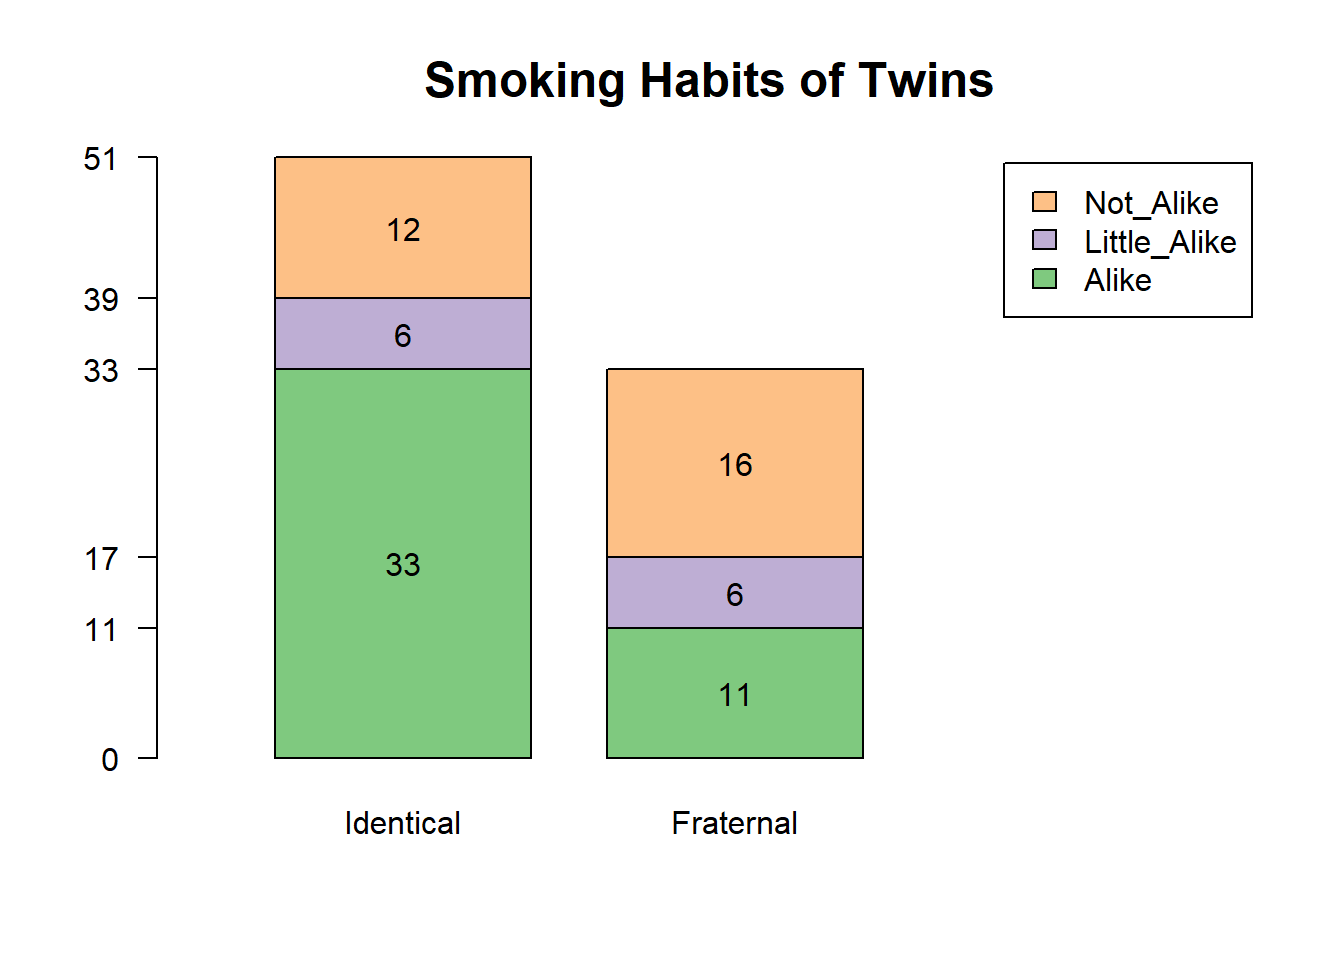
\includegraphics{Nightingale_Coxcomb_files/figure-latex/unnamed-chunk-3-1.pdf}

\begin{Shaded}
\begin{Highlighting}[]
\KeywordTok{ggsave}\NormalTok{(cxc_b, }\DataTypeTok{file =} \StringTok{"../pics/cxc_b.png"}\NormalTok{, }\DataTypeTok{width =} \DecValTok{12}\NormalTok{, }\DataTypeTok{height =} \DecValTok{7}\NormalTok{)}
\end{Highlighting}
\end{Shaded}

\hypertarget{coxcomb-plot}{%
\subsection{Coxcomb Plot}\label{coxcomb-plot}}

\begin{Shaded}
\begin{Highlighting}[]
\NormalTok{cxc1 <-}\StringTok{ }
\StringTok{  }\KeywordTok{ggplot}\NormalTok{(}\DataTypeTok{data =}\NormalTok{ Night }\OperatorTok\StringTok{ }\KeywordTok{subset}\NormalTok{(Regime }\OperatorTok{==}\StringTok{ "Before"}\NormalTok{),}
         \KeywordTok{aes}\NormalTok{(}\DataTypeTok{x =}\NormalTok{ Month, }
             \DataTypeTok{y =}\NormalTok{ Deaths, }
             \DataTypeTok{fill =}\NormalTok{ Cause)) }\OperatorTok{+}
\StringTok{  }\KeywordTok{geom_bar}\NormalTok{(}\DataTypeTok{width =} \DecValTok{1}\NormalTok{, }
           \DataTypeTok{stat =} \StringTok{"identity"}\NormalTok{, }
           \DataTypeTok{position =} \StringTok{"stack"}\NormalTok{, }
           \DataTypeTok{colour =} \StringTok{"black"}\NormalTok{) }\OperatorTok{+}
\StringTok{  }\KeywordTok{scale_y_sqrt}\NormalTok{() }\OperatorTok{+}
\StringTok{  }\KeywordTok{coord_polar}\NormalTok{(}\DataTypeTok{start =} \DecValTok{3} \OperatorTok{*}\StringTok{ }\NormalTok{pi }\OperatorTok{/}\StringTok{ }\DecValTok{2}\NormalTok{)}
\NormalTok{cxc1}
\end{Highlighting}
\end{Shaded}

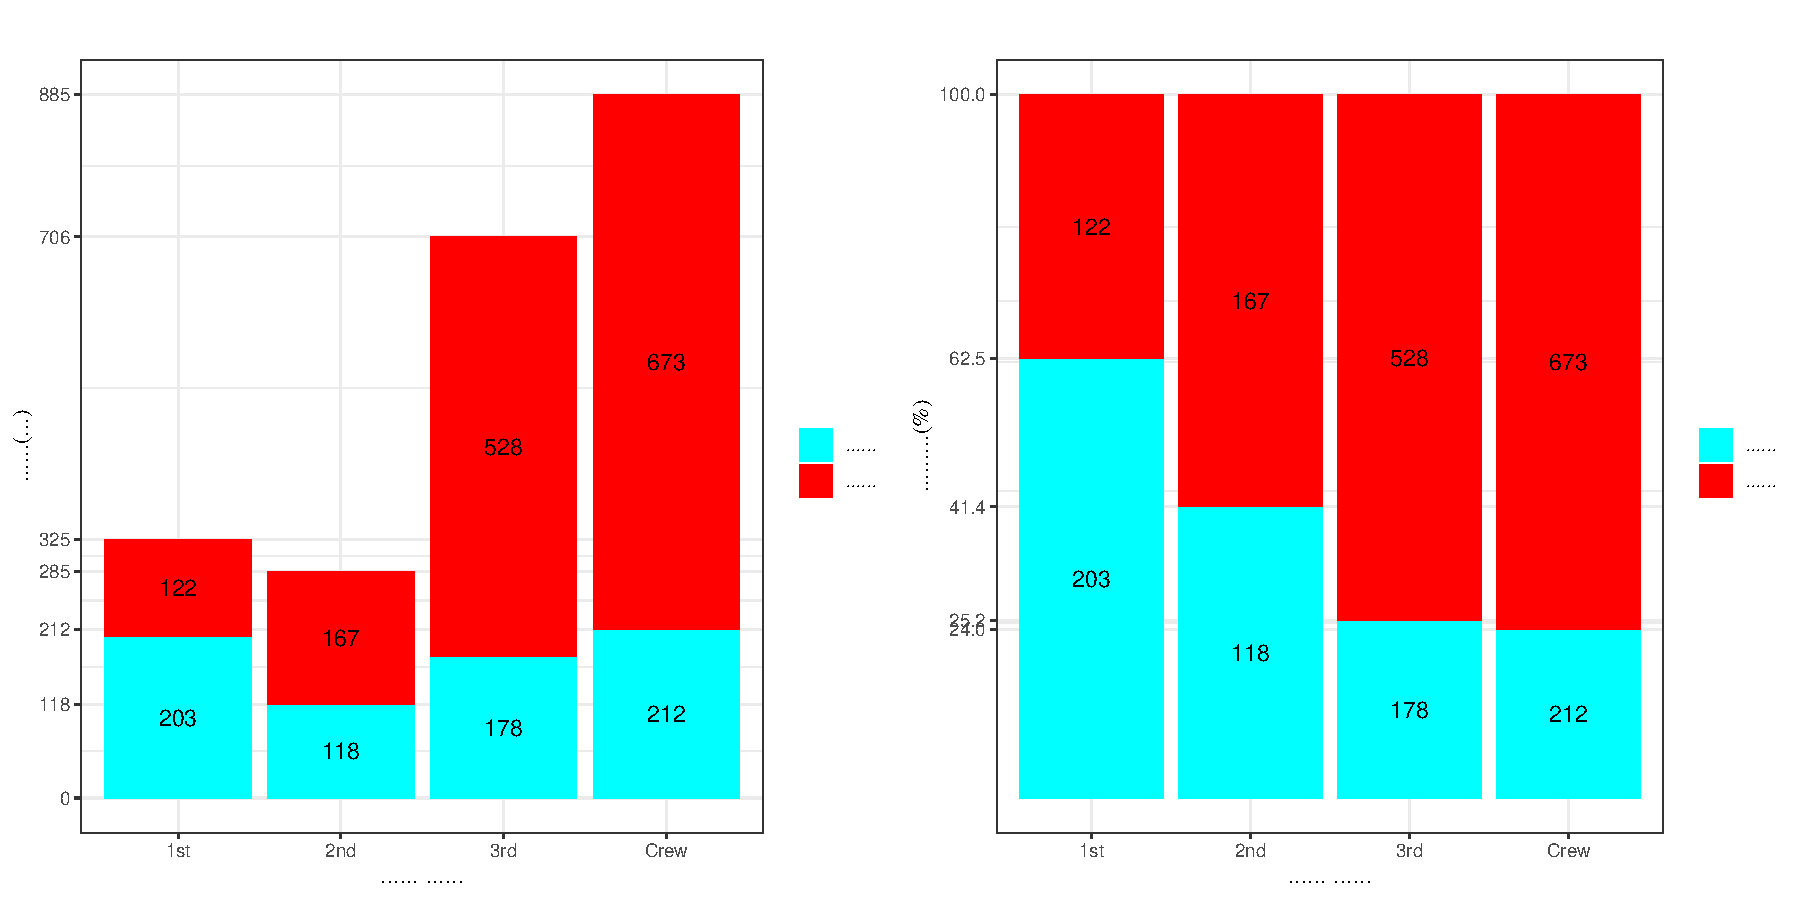
\includegraphics{Nightingale_Coxcomb_files/figure-latex/unnamed-chunk-4-1.pdf}

\begin{Shaded}
\begin{Highlighting}[]
\NormalTok{cxc2 <-}\StringTok{ }
\StringTok{  }\KeywordTok{ggplot}\NormalTok{(}\DataTypeTok{data =}\NormalTok{ Night }\OperatorTok\StringTok{ }\KeywordTok{subset}\NormalTok{(Regime }\OperatorTok{==}\StringTok{ "After"}\NormalTok{),}
         \KeywordTok{aes}\NormalTok{(}\DataTypeTok{x =}\NormalTok{ Month, }
             \DataTypeTok{y =}\NormalTok{ Deaths, }
             \DataTypeTok{fill =}\NormalTok{ Cause)) }\OperatorTok{+}
\StringTok{  }\KeywordTok{geom_bar}\NormalTok{(}\DataTypeTok{width =} \DecValTok{1}\NormalTok{, }
           \DataTypeTok{stat =} \StringTok{"identity"}\NormalTok{, }
           \DataTypeTok{position =} \StringTok{"stack"}\NormalTok{, }
           \DataTypeTok{colour =} \StringTok{"black"}\NormalTok{) }\OperatorTok{+}
\StringTok{  }\KeywordTok{scale_y_sqrt}\NormalTok{() }\OperatorTok{+}
\StringTok{  }\KeywordTok{coord_polar}\NormalTok{(}\DataTypeTok{start =} \DecValTok{3} \OperatorTok{*}\StringTok{ }\NormalTok{pi }\OperatorTok{/}\StringTok{ }\DecValTok{2}\NormalTok{)}
\NormalTok{cxc2}
\end{Highlighting}
\end{Shaded}

\includegraphics{Nightingale_Coxcomb_files/figure-latex/unnamed-chunk-4-2.pdf}

\hypertarget{facet}{%
\subsection{facet}\label{facet}}

\begin{Shaded}
\begin{Highlighting}[]
\NormalTok{Regime_lab <-}\StringTok{ }\KeywordTok{c}\NormalTok{(}\StringTok{"Before"}\NormalTok{, }\StringTok{"After"}\NormalTok{)}
\KeywordTok{names}\NormalTok{(Regime_lab) <-}\StringTok{ }\KeywordTok{c}\NormalTok{(}\StringTok{"Before"}\NormalTok{, }\StringTok{"After"}\NormalTok{)}
\NormalTok{cxc_f <-}\StringTok{ }
\StringTok{  }\KeywordTok{ggplot}\NormalTok{(}\DataTypeTok{data =}\NormalTok{ Night,}
         \KeywordTok{aes}\NormalTok{(}\DataTypeTok{x =}\NormalTok{ Month, }
             \DataTypeTok{y =}\NormalTok{ Deaths, }
             \DataTypeTok{fill =}\NormalTok{ Cause)) }\OperatorTok{+}
\StringTok{  }\KeywordTok{geom_bar}\NormalTok{(}\DataTypeTok{width =} \DecValTok{1}\NormalTok{, }
           \DataTypeTok{stat =} \StringTok{"identity"}\NormalTok{, }
           \DataTypeTok{position =} \StringTok{"stack"}\NormalTok{, }
           \DataTypeTok{colour =} \StringTok{"black"}\NormalTok{) }\OperatorTok{+}
\StringTok{  }\KeywordTok{scale_y_sqrt}\NormalTok{() }\OperatorTok{+}
\StringTok{  }\KeywordTok{scale_fill_brewer}\NormalTok{(}\DataTypeTok{type =} \StringTok{"qual"}\NormalTok{, }\DataTypeTok{palette =} \StringTok{"Pastel2"}\NormalTok{) }\OperatorTok{+}
\StringTok{  }\KeywordTok{facet_grid}\NormalTok{(. }\OperatorTok{~}\StringTok{ }\NormalTok{Regime, }
             \DataTypeTok{scales =} \StringTok{"fixed"}\NormalTok{, }
             \DataTypeTok{labeller =} \KeywordTok{labeller}\NormalTok{(}\DataTypeTok{Regime =}\NormalTok{ Regime_lab)) }\OperatorTok{+}
\StringTok{  }\KeywordTok{coord_polar}\NormalTok{(}\DataTypeTok{start =} \DecValTok{3} \OperatorTok{*}\StringTok{ }\NormalTok{pi }\OperatorTok{/}\StringTok{ }\DecValTok{2}\NormalTok{)}
\NormalTok{cxc_f}
\end{Highlighting}
\end{Shaded}

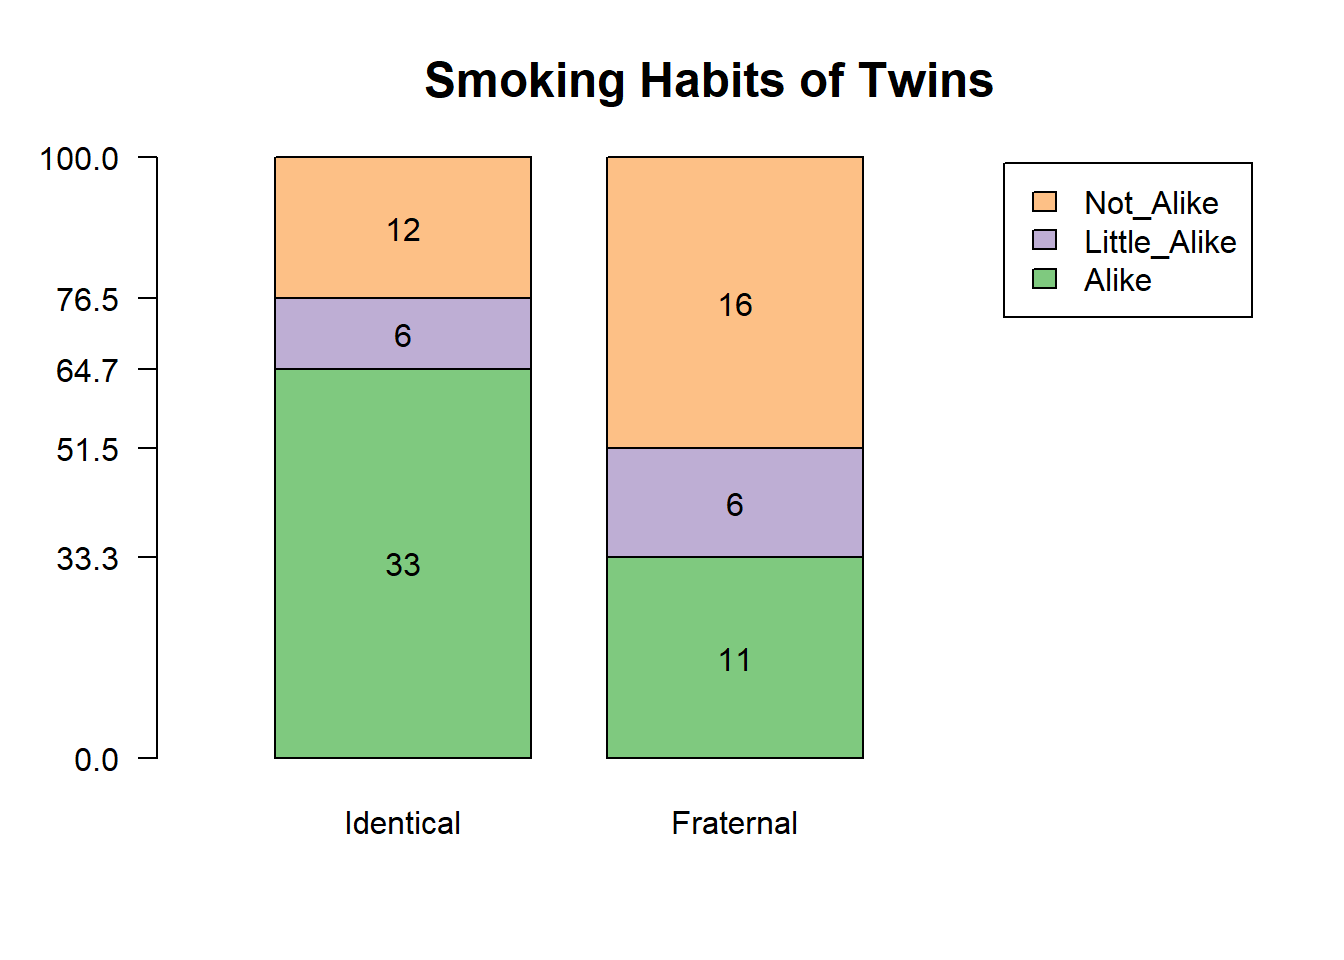
\includegraphics{Nightingale_Coxcomb_files/figure-latex/unnamed-chunk-5-1.pdf}

\begin{Shaded}
\begin{Highlighting}[]
\KeywordTok{ggsave}\NormalTok{(cxc_f, }\DataTypeTok{file =} \StringTok{"../pics/cxc_f.png"}\NormalTok{, }\DataTypeTok{width =} \DecValTok{12}\NormalTok{, }\DataTypeTok{height =} \DecValTok{7}\NormalTok{)}
\end{Highlighting}
\end{Shaded}

\end{document}
